\documentclass{myclass}

\setmytitle{pre-course lecture}
\setmysubtitle{script}

\begin{document}

\makemytitle


%%%%%%%%%%%%%%%%
%%% 1. Day 1 %%%
%%%%%%%%%%%%%%%%

\begin{important}[TODO:]
	Which of the following is the best:
	\[ a \times b \]
	\begin{verbatim}
		( a \times b )
	\end{verbatim}
	\vspace{0.5cm}
	\[ a \cdot b \]
	\begin{verbatim}
		( a \cdot b )
	\end{verbatim}
	\vspace{0.5cm}
	\[ a \ast b \]
	\begin{verbatim}
		( a \ast b )
	\end{verbatim}
	\vspace{0.5cm}
	( \verb|\times| can be redefined to any symbol )
\end{important}

\section{Day 1}
Argumente/Begründungen/Beweise (Herz der Mathematik)\\
Beweise sind ``immer wahr''\\
Beweise helfen beim verstehen\\
Beweise ``zähmen die Unendlichkeit''\par

\begin{problem}
	Wie lange benötigt man zum Zersägen eines $\qty{7}{\meter}$-langen Baumstamms in $\qty{1}{\meter}$-Stücke, wenn jeder Schnitt eine halbe Minute dauert?\par
	Lsg.: $\qty{3}{\minute}$\par
	Zwischenziel: 6 Schritte $\rightarrow$ Mustererkennung $n-1$ Schnitte für $n$ Teiler/Meter\par
	\begin{proof}
		Jeder Schnitt erhöht die Anzahl der Stücke um eins.\par
		Anfangs: $1$ Stück, am Ende $7$ $\Rightarrow$ man muss \[7 - 1 = 6 \text{ Schnitte machen. usw.}\]
	\end{proof}
\end{problem}

$\mathbb{N} = \{1, 2, 3, ...\} \text{ natürliche Zahlen}$\\
$\mathbb{N}_0 = \{0, 1, 2, ...\} \text{ natürliche Zahlen mit der Null}$\par

\begin{problem}
	\begin{conjecture}
		Wenn zwei natürliche Zahlen gerade sind, dann ist auch ihre Summe gerade
	\end{conjecture}
	Seien $t_1, t_2 \in \mathbb{N}$
	\[ a = 2t_1 \]
	\[ b = 2t_2 \]
	also gilt:
	\[ a + b = 2t_1 + 2_t2 = 2(t_1+t_2) \implies \text{ gerade Zahl}\]
\end{problem}

\begin{problem}
	Mit wievielen Nullen endet $100!$?\par
	Primfaktorzerlegung:\\
	$20$ durch $5$ teilbare Zahlen\\
	$4$ durch $5^2$ teilbare Zahlen\par
	$k$ Nullen am Ende einer natürlichen Zahl in Dezimalschreibweise: Zahl ist durch $10^k = \left( 2 \times 5 \right)^k = 2^k  \times 5^k$ teilbar.
	\[5, 10, 15, ...\]
	also bei
	\[1 \times 5, 2 \times 5, 3 \times 5, ..., 20 \times 5 \Rightarrow \qty{20}{\text{Stück}}\]
	welche liefern $2$ Fünfen
	\[1 \times 5^2, 2 \times 5^2, 3 \times 5^2, 4 \times 5^2, \text{\hbox{\sout{$5 \times 5^2$}}}\]\par
	Anzahl der Nullen, mit denen $100!$ enden, ist die größte natürliche Zahl $k \in \mathbb{N}$, für die
	\[100! \text{ durch } 10^k \text{ teilbar ist.}\]
	Weil $10 = (2 \times 5)$, ist das gleich der größten ganzen Zahl $k$, für die $100!$ durch $2^k \times 5^k$ teilbar ist,
	\[\text{also durch } 5^k \text{ und } 2^k\]
	Die $5$ tritt als Faktor genau in den $20$ Zahlen
	\[5, 10, 15, ..., 100,\]
	und in den $4$ Zahlen
	\[25, 50, 75, 100\]
	doppelt vor.\\
	Somit folgt: die $5$ tritt $20 + 4 = 24$ mal als Faktor in $100!$ auf.\\
	Die $2$ tritt als Faktor in $50$ Zahlen auf:
	\[2, 4, 6, 8, ..., 100\]
	(und einigen mehrfach)\\
	$\Rightarrow$ Insgesamt endet $100!$ mit $24$ Nullen.
\end{problem}

\begin{problem}
	Es sei $n \in \mathbb{N}$. Berechne die Summe der ersten $n$ natürlichen Zahlen, also
	\begin{alignat*}{7}
		&~{}	&&1		&&+ 2		&&+ 3		&&+ ... &&+ n			&&\coloneqq S\\
		&+{} 	&&n		&&+ n - 1	&&+ n - 2	&&+ ... &&+ 1			&&= S\\
		\hline
		&={} 	&&(n+1)		&&+(n+1)	&&+(n+1)	&&+ ... &&+(n+1)		&&= S\\
		&={} 	&&~		&&~		&&~		&&~	&&n\times (n + 1)	&&= S
	\end{alignat*}
\end{problem}

\section{Tag 2}
$\mathbb{P} = \text{Menge aller Primzahlen}$\\
$\mathbb{P} = {2, 3, 5, 7, ...}$\\
Offene Fragen: Gibt es eine Formel für Primzahlen?\\
Fermat (1637):
\begin{conjecture}
	$F(n) = 2^{2^n} + $ ist eine Primzahl für jedes $n \in \mathbb{N}$
	\begin{alignat*}{3}
		F(1) &= 2^{2^1} + 1 &&= 2^2 + 1 &&= 5\\
		F(2) &= 2^{2^2} + 1 &&= 2^4 + 1 &&= 17\\
		F(3) &= 2^{2^3} + 1 &&= 2^8 + 1 &&= 257\\
		F(4) &= 2^{2^4} + 1 &&= 2^{16} + 1 &&= 65537
	\end{alignat*}
\end{conjecture}
100 Jahre später Euler:\\
$651$ teilt $F(5)$,\\
also ist
\[F(5) = 4294967297\]
\underline{keine} Primzahl.

\section{Vorkurs}
\begin{itemize}
	\item mathematische Probleme formulieren
	\item Lösungen finden (Argumentieren) Beweisen
\end{itemize}

\section{Mengen (Warm-up)}
Skatspiel\par
Situation: Aus gemischtem Skatspiel werden zwei Karten gezogen. Sind es zwei Karten gleicher Farbe oder zwei Karten mit gleichem Wert, dann gewinnen wir.\par
Symbole: Kreuz, Pik, Herz, Karo\par
Werte: 7, 8, 9, 10, B, D, K, Ass\par
Definitionssymbol: `` $\coloneqq$ ''\par
\begin{example}
	\begin{align*}
		11 &\coloneqq \text{Bube}	& a &\coloneqq \text{Kreuz}\\
		12 &\coloneqq \text{Dame}	& b &\coloneqq \text{Pik}\\
		13 &\coloneqq \text{König}	& c &\coloneqq \text{Herz}\\
		14 &\coloneqq \text{Ass}	& d &\coloneqq \text{Karo}
	\end{align*}
	$\text{Kartenmenge} = \left\{a7, a8, ..., a14, b7, b8, ..., b14, c7, ..., d14\right\}$\\
	$\left\{\text{Kreuz, 7}\right\} = \text{Karte Kreuz 7}$
	\begin{alignat*}{4}
		\text{Kartenmenge} \coloneqq \{	&\{1, 7\}, &&\{2, 7\}, &&\{3, 7\}, &&\{4, 7\}\\
		~				&\{1, 8\}, &&\{2, 8\}, &&\{3, 8\}, &&\{4, 8\}, ...,\\
		~				&\{1, 14\}, &&\{2, 14\}, &&\{3, 14\}, &&\{4, 14\}\}
	\end{alignat*}
\end{example}


%%%%%%%%%%%%%%%%%%%%%%%%%%%%%%%%%%%%%%%%%%%%%%%%
%%% 5. Mengen, Teilmengen, Mengenoperationen %%%
%%%%%%%%%%%%%%%%%%%%%%%%%%%%%%%%%%%%%%%%%%%%%%%%

\section{Mengen, Teilmengen, Mengenoperationen}

\begin{definition}
	(naive Definition) Eine Ansammlung von (mathematischen) Objekten heißt \textbf{Menge}. Ein Mitglied dieser Ansammlung heißt \textbf{Element} der Menge.
\end{definition}

Ist $a$ ein Element der Menge $A$, so schreibt man $a \in A$\par
Gehört $a$ nicht zur Menge $A$, so schreibt man $a \notin A$\\
Mit $\vert A \vert$ bezeichnet man die Anzahl der Elemente in $A$

\begin{example}
	\[\vert\mathbb{N}\vert=\infty\]
\end{example}

Zwei Arten, Mengen zu beschreiben:

\begin{itemize}
	\item aufzählende Mengenschreibweise $A = \{2, 4, 6, ...\}$, $B = \{2, 8, 9\}$
	\item beschreibende Mengenschreibweise $A = \{x \in \mathbb{N} \vert 3 \leq x \leq 8\}$, $[a, b] \coloneqq \{z \in \mathbb{R} \vert a \leq z \leq b \} a,b \in \mathbb{R}$
\end{itemize}

\begin{task}
	\begin{align*}
		M &= \text{Menge aller ganzzahlingen Vielfachen von 42}\\
		~ &= \{x \in \mathbb{Z} : 42\vert x\} = \{42\times x : x \in \mathbb{Z}\}
	\end{align*}
	\begin{definition}
		Es sei $A$ eine Menge\\
		Eine Menge $B$ heißt Teilmenge von $A$, in Zeichen: $B \subseteq A$,\\
		wenn jedes Element von $B$ auch ein Element von $A$ ist
	\end{definition}
	\begin{definition}
		Es seien $A, B$ Teilmengen einer Menge $M$\\
		Schnittmenge von $A$ und $B$ ist $A \cap B \coloneqq \{x \in M : x\in A \wedge x \in B\}$\\
		Vereinigungsmenge von $A$ und $B$ ist $A \cup B \coloneqq \{x \in M : x\in A \vee x \in B\}$\\
		Differenz von $A$ und $B$ ist $A \backslash B \coloneqq \{x \in M : x\in A \wedge x \notin B\}$\\
		Komponent von $A$ in $M$ ist die Menge $A^c \coloneqq \{x \in M : x \notin A \} = M \backslash A\}$\\
		genau dann wenn $A \subseteq B$ und $B \subseteq A$, dann $A = B$
	\end{definition}
\end{task}
Jede beliebeige Menge $A$ hat die folgenden Teilmengen $\emptyset, A$ d.h. es git $\emptyset \subseteq A,A \subseteq A$\\
$\{\_\} \notin \{\_,\_\}$\\
$\_ \in \{\square, \circ, \triangle\}$ (bzw. $\_ \in \{\_, \_, \_\}$)\\
$\{1, 2, 3\} = \{3, 2, 1\} = \{2, 1, 3\} = ...$
\begin{task}
	Gilt $\{1, 2, 1, 1\} = \{1, 2\}$?\\
	\indent\indent ja
\end{task}
\begin{task}
	Falls $\{a\} = \{b\}$, dann folgt $a = b$\\
	Falls $\{a\} = \{a, b\}$, dann folgt $a = b$
\end{task}
$\{1, 2\}$ hat Teilmengen $\emptyset, \{1\}, \{2\}, \{1, 2\}$\\
Eine Menge mit $n$ Elementen hat $2^n$ Teilmengen.
\begin{definition}
	Potenzmenge einer Menge\\
	Sei $A$ eine Menge, dann heißt die Menge
	\[\mathcal{P}(A)\]
	aller Teilmengen von $A$ die \underline{Potenzmenge von $A$}
\end{definition}
$\mathcal{P}(\emptyset) = \{\emptyset\}\:\mathcal{P}(\{1\}) = \{\emptyset, 1\}$
\begin{definition}
	(kartesisches Produkt von zwei Mengen $A$ und $B$)\\
	Das kartesische Produkt von zwei Mengen $A$ und $B$ ist definiert durch
	\[A \times B \coloneqq \{(x,y): x \in A \wedge y \in B\}\]
	In $A \times B$ sind zwei Elemente $(x_1, y_1), (x_2, y_2)$ genau dann gleich, wenn $x_1 = x_2$ und $y_1 = y_2$
	\[\mathbb{R}^2 \coloneqq \mathbb{R} \times \mathbb{R} = \{(x, y): x, y \in \mathbb{R}\]
	\indent\indent $(1,2) \in \mathbb{R}^2 \qquad (1,2) \neq (2,1)$\\
	\indent\indent $(2,1) \in \mathbb{R}^2$
\end{definition}

\section{Prof. Junk}
Auf einem Baum saß ein Rabe mit einem Käse im Schnabel, als ein Fuchs vorbeikommt.\\
Sei $B \in \text{Bäume}$ und $R \in \text{Raben}$ sitze auf $B$ mit $K \in \text{Käsestückchen}$ im Schnabel, als $F \in \text{Füchse}$ vorbeikommt.\par
Er überlegte wie er an den Käse kommt. Da sagte er zu dem Raben, ...\\
$F$ überlegte wie $F$ an $K$ kommt. Da sagte $F$ zu $R$, ...\par

allgemeine mathematische Situationen bestehen aus
\begin{itemize}
	\item Eine Liste von Namen für mathematische Objekte
	\item Eine Liste von geltenden Aussagen über diese Objekte
\end{itemize}
Was kann man damit tun?
\begin{itemize}
	\item Namen kann man austauschen ohne Bedeutungsänderung
	\item Situationen können \underline{eintreten}; konkrete Situationen können auf allgemeine Situationen passen
\end{itemize}

\begin{example}
	$A \coloneqq \{ x \in \mathbb{N} : 3 \leq x \leq 8\}$\\
	Schreibweise beschreib eine Menge, indem sie zwei Zugehörigkeits\underline{regeln} kodiert
	\begin{itemize}
		\item besteht aus zwei allgemeinen Situationen:
			\begin{itemize}
				\item Vorraussetzung
				\item Folgerung
			\end{itemize}
	\end{itemize}
	Regel 1: Sei $x$ ein Objekt\\
	Es gelte $x \in \mathbb{N}; 3 \leq; 8 \geq x \rightarrow$ Dann gilt $x \in A$\\
	Regel 2: Sei $x$ ein Objekt\\
	Es gelte  $x \in A\rightarrow$ Dann gilt $x \in \mathbb{N}; 3 \leq; 8 \geq x$\\
	\indent Gilt: $9 \in A$:\quad$x \leftarrow 9$
	\indent\indent $9 \in \mathbb{N}, 9 \geq 3, 9 \leq 8$\\
	\indent\indent Vorraussetzung tritt nicht ein!
	\indent Gilt: $9 \notin A$
	\indent\indent $9 \in \mathbb{N}, 9 \geq 3, 9 \leq 8 \rightarrow$ Wiederspruch\\
	\indent\indent\indent $9 \nleq 8\rightarrow$ Gegenteil von Annahme stimmt
\end{example}

\section{Aussagen (Logik)}
Unsere mathematische Ergebnisse formulieren wir als (mathematische) Aussagen.\\
Als Aussage bezeichnen wir einen Ausdruck, der entweder wahr oder falsch sein kann.\\
$\rightsquigarrow$ Wahrheitswert der Aussage: wahr, w, $1$; falsch, f, $0$
\begin{example}
	\begin{align*}
		A &\coloneqq \text{ ``$1+2=3$''}\\
		B &\coloneqq \text{ ``$5$ ist eine negative Zahl''}\\
		C &\coloneqq \text{ ``Jede gerade Zahl $n > 2$ kann als Sume zweier Primzahlen geschrieben werden.''}
	\end{align*}
\end{example}


%%%%%%%%%%%%%%%%%%%%%%
%%% 8. Aussageform %%%
%%%%%%%%%%%%%%%%%%%%%%

\section{Aussageform}

\begin{example}
	Sei
	\[ A(n) \coloneqq n \text{ ist gerade}\]
	Dann ist
	\[ A(1) \text{ eine (falsche) Aussage}\]
	\[ A(2) \text{ eine (wahre) Aussage}\]
\end{example}

Eine Aussageform ist eine Äußerung, die eine (oder mehrere) Variablen enthält und zu einer Aussage wird, wenn man zulässige Objekte für diese Variablen einsetzt.\\
Es seien $A$ und $B$ Aussagen.\par
Die Konjunktion (Und-Aussage) von $A$ und $B$ ist die Aussage
\[ A \land B \text{ ``$A$ und $B$''}\]
die genau dann wahr ist, wenn $A$ und $B$ gleichzeitig wahr sind.
\[ A \coloneqq \text{ ``$24$ ist gerade''}\]
\[ B \coloneqq \text{ ``$24$ ist durch $3$ teilbar''}\]
\[ C \coloneqq \text{ ``$24$ ist durch $5$ teilbar''}\]
\[ A \land B = 1\quad A \land C = 0\]
Die Disjunktion (Oder-Aussage) von $A$ und $B$ ist Aussage
\[A \lor B \text{ ``$A$ oder $B$''}\]
die genau dann wahr ist, wenn mind. eine der beiden Aussagen $A$ und $B$ wahr ist.\par
Die Negation von $A$ ist die Aussage
\[ \neg A \text{ ``nicht A''}\]
die genau dann wahr ist, wenn $A$ falsch ist.\par
Implikation (Folgerung) ``Wenn $A$, dann $B$'' ist die Aussage
\[ A \implies B \text{ ``aus $A$ folgt $B$'', $A$ impliziert $B$'')}\]
die genau dann falsch ist, wenn $A$ wahr ist und $B$ falsch ist und sonst ist sie immer wahr.\par
Äquivalenz ``A genau dann, wenn B'' ist die Aussage
\[ A \iff B \]
die genau dann wahr ist, wenn $A$ und $B$ beide wahr sind oder $A$ und $B$ beide falsch sind.\par
Eine zusammengesetzte Aussage heißt \underline{Tautologie,} falls sie immer wahr ist, unabhängig davon, welche Wahrheitswerte die verknüpften Einzelaussagen haben.\par

Ist  $A(n)$ eine Aussageform mit Wertebereich $M$, so können wir folgende Aussagen betrachten:
\begin{itemize}
	\item für alle $n \in M$ gilt: $A(n)$\\
		in Zeichen: $\forall n \in M : A(n)$ z.B. $\forall n \in \mathbb{N}: 2 \mid n$\\
		$\rightarrow$ Allaussage ($\forall \leftarrow$ Allquantor)
	\item Es gibt ein $n \in M$, für das $A(n)$ gilt\\
		in Zeichen $\exists n \in M : A(n)$\\
		\quad $\exists! n \in M : A(n)$ ``es gibt genau ein $n \in M, ...$''
	\item Eine Aussage der Form
		\[\forall n \in M : A(n)\]
		ist immer wahr, wenn $M = \{\}$
	\item Reihenfolge der Quantoren spielt eine Rolle
		\[A : \forall n \in \mathbb{N}: (\exists m \in \mathbb{N}: m > n)\text{ (wahr)}\]
		\[B : \exists m \in \mathbb{N}: \forall n \in \mathbb{N}: m > n\text{ (falsch)}\]
\end{itemize}


%%%%%%%%%%%%%%%%%%%%%%%%%%%%%%%%
%%% 9. Negation von Aussagen %%%
%%%%%%%%%%%%%%%%%%%%%%%%%%%%%%%%

\section{Negation von Aussagen}
$\neg (\exists n \in M : A(n)) \iff \forall n \in M : \neg A(n)\quad\text{ist eine Tautologie}$
d.h. die Negation der Aussage
\[ \exists n \in M : A(n) \]
ist logisch Äquivalent zu der Aussage
\[ \forall n \in M : \neg A(n) \]

$\neg ( \forall n \in M : A(n)) \iff \exists n \in M : \neg A(n)\quad\text{ist eine Tautologie}$
d.h. die Negation der Aussage
\[ \forall n \in M : A(n) \]
ist logisch Äquivalent zu der Aussage
\[ \exists n \in M : \neg A(n) \]

\section{---}
\begin{theorem}
	\begin{enumerate}[label=\arabic*)]
		\item Äquivalenzprinzip\\
			Ist A wahr und ist $A \iff B$, dann ist auch $B$ wahr
		\item Ableitungsregel\\
			$(A \land (A \implies B)) \implies B$ ist eine Tautologie
		\item Syllogismusregel\\
			$((A \implies B) \land (B \implies C)) \implies A \;\implies\; C$ ist eine Tautologie
		\item Kontraposition\\
			$(A \implies B) \iff (\neg B \implies \neg A)$ ist eine Tautologie
		\item Ringschluss
			\begin{equation*}
				((A \iff B) \land (B \iff C) \land (A \iff C))
			\end{equation*}
			\begin{equation*}
				\iff
			\end{equation*}
			\begin{equation*}
				((A \iff B) \land (B \iff C) \land (A \iff C))
			\end{equation*}
	\end{enumerate}
\end{theorem}


%%%%%%%%%%%%%%%%%%%%%%%%%%%%%%%%%%%%
%%% 11. Beweise und Beweisformen %%%
%%%%%%%%%%%%%%%%%%%%%%%%%%%%%%%%%%%%
\section{Beweise und Beweisformen}

Ein Beweis ist eine logisch vollständige Begründung einer Aussage. Oft möchten wir Aussagen vom Typ ``Wenn A, dann B'' zeigen.\\
Aussagen lassen sich meist in folgende Form bringen
\begin{itemize}
	\item Vorraussetzung z.B. Sei $a \in \mathbb{N}$.
	\item Behauptung\quad\quad\quad\quad dann ist $2 = \text{gerade}$
\end{itemize}

%%% Direkter Beweis %%%
\subsection{Direkter Beweis}
Statt $A \implies B$ zu zeigen, zeigen wir $A \implies A_1 \implies A_2 \implies ... \implies B$\par
Situation: $\mathbb{N} = \{1, 2, ... \}, \mathbb{N}_0 = \{0, 1, 2, ... \}$, Rechenregeln: $+$, $-$ bekannt
\begin{subdefinition}
	Eine natürliche Zahl $b \in \mathbb{N}$ teilt eine natürliche Zahl $a \in \mathbb{N}$ (in Zeichen $b \mid a$), wenn es eine natürliche Zahl $c \in \mathbb{N}$ gibt, mit $a = b \times c$
\end{subdefinition}
\begin{subdefinition}
	\label{subdefgeradezahl}
	Eine Zahl $a \in \mathbb{N}$ heißt \underline{gerade}, falls $2\mid a$ gilt, d.h. falls es ein $c \in \mathbb{N}$ mmit $a = 2 \times c$ gibt.\\
	Eine Zahl $q \in \mathbb{N}$ heißt \underline{ungerade}, falls $q$ nicht gerade ist.
\end{subdefinition}
\begin{subconjecture}
	$18$ ist gerade.
	\begin{subproof}
		$18 \in \mathbb{N}$, also können wir obrige Definition \ref{subdefgeradezahl} anwenden.\\
		Setze $c \coloneqq 9$\\
		Dann gilt $c \in \mathbb{N}$ und $18 = 2 \times 9$\\
		Also gilt $2 \mid 18$. Also ist $18$ gerade, $\square$
	\end{subproof}
\end{subconjecture}


%%%%%%%%%%%%%%%%%%%%%%%%%%%%%%%%%
%%% Apendix B von Junk/Traude %%%
%%%%%%%%%%%%%%%%%%%%%%%%%%%%%%%%%

\section{Apendix B von Junk/Traude}
\begin{definition}[\fbox{B.10} Definitionen]
	\label{def:B.10}
	\begin{enumerate}[label=]
		\item Nachweistext: Definition $\bigstar$ wird \fbox{Blubb} genannt, falls \circled{...} gilt.\\
			Schreibe: Zu zeigen \circled{...}
		\item Benutzungsbedingung: um zu benutzen, dass ein Objekt nach Definition $\bigstar$ Blubb genannt wird, falls \circled{...} gilt.\\
			Schreibe: Nach Definition von ``Blubb'', folgt \circled{...}
	\end{enumerate}
	\fbox{B.7} Existenzaussagen
	\begin{enumerate}[label=]
		\item Nachweistext: zu beweisen:
			\[ \exists x \in X : \circled{\text{...}} \]
			Schreibe:
			\begin{enumerate}[label=]
				\item Setze $x \coloneqq \_ \_ \_$.
				\item zu zeigen: $ x \in X$ mit \circled{...}
			\end{enumerate}
		\item Benutzungstext: Es gilt
	\end{enumerate}
	\begin{example}
		Vor. Sei $a \in \mathbb{N}$\\
		Bew. Dann ist $2 \times a$ gerade\par
		Es sei $a \in \mathbb{N}$. Es gilt $2 \times a \in \mathbb{N}$. Nach Definition \ref{subdefgeradezahl} zu geraden Zahlen ist zu zeigen:
		\[ 2 \mid a \]
		d.h. zu zeigen: $ \exists c \in \mathbb{N} : s \times a = 2 \times c $\\
		Setzte $ c \coloneqq a $\\
		Dann gilt $ c \in \mathbb{N} $ und
		\[ 2 \times a = 2 \times c, \square \]
	\end{example}
\end{definition}

\begin{definition}[\fbox{B.6} Allaussagen]
	\label{def:B.6}
	Nachweistext: zu zeigen
	\[ \forall x \in X : \text{\circled{...}} \]
	\begin{indentpar}
		\indent Schreibe:\\
		Sei ein $ x \in X $ gegeben.\\
		Zeige: \circled{...}
	\end{indentpar}
	Benutzungstext:
	\begin{equation}
		\label{B.6.1}
		\forall x \in X : \text{\circled{...}} \text anzuwenden
	\end{equation}
	Dann muss ein $ a \in X $ vorliegen\\
	Wegen $ a \in X $ folgt (aus der $\forall$-Aussage)\\
	\indent\circled{...}
\end{definition}

\begin{task}
	Zeige, dass die Summe zweier geraden natürlichen Zahlen auch gerade ist\par
	Vor.: Gegeben seien $ a \in \mathbb{N} $ und $ b \in \mathbb{N} $ gerade.\\
	Setzte
	\[ c \coloneqq a + b \in \mathbb{N} \]
	Beh.: $c$ ist gerade
	\begin{proof}
		Da $ c \in \mathbb{N} $, kann man Definition \ref{subdefgeradezahl} zu geraden Zahlen anwenden. Zu zeigen ist
		\[ 2 \mid c \]
		d.h. zu zeigen: $ \exists k \in \mathbb{N} : c = 2 \times k $\par
		Da $a, b$ gerade, gilt nach Definition \ref{subdefgeradezahl} zu geraden Zahlen
		\begin{equation}
			\label{exampleone}
			a = 2 \times m \text{ und}
		\end{equation}
		\begin{equation}
			\label{exampletwo}
			b = 2 \times n,
		\end{equation}
		mit $ m, n \in \mathbb{N} $, sodass
		\begin{equation}
			\label{examplethree}
			c = a + b = 2 \times m + 2 \times n = 2 \times ( m + n ),
		\end{equation}
		wobei wir für die erste Gleicheit \ref{exampleone} und \ref{exampletwo}, für die zweite Gleichheit die Rechenregeln für natürliche Zahlen benutzt haben.\\
		Setze
		\[ k \coloneqq m + n \]
		Dann gilt
		\[ k \in \mathbb{N} \]
		und wegen \ref{examplethree}
		\[ c = 2 \times ( m + n ) \]
		also
		\[
			c = 2 \times k, \tag*{$\square$}
		\]
	\end{proof}
\end{task}

\begin{definition}[`` $\mid$ '']
	\label{def:mid}
	$ a, b \in \mathbb{N} $\\
	$ b \mid a $, falls es $ c \in \mathbb{N} $ mit $ a = b \times c $ gibt.
\end{definition}
	$\Downarrow$\\
	$ a, b, c \in \mathbb{N} $\\
	$ b \times c \mid a \times c $, falls es $ n \in \mathbb{N} $ mit $ a \times c = ( b \times c ) \times n $ gibt.

\begin{task}[Es seien $a, b \in \mathbb{N}$. Weiter gelte $ b \mid a $. Dann gilt auch $ b \times c \mid a \times c $]
	\begin{proof}[Vor.: Es seien $ a, b \in \mathbb{N} $ mit $ b \mid a $]
		z.z.: $ ( b \times c ) \mid ( a \times c ) $\\
		d.h.: z.z.: es existiert $ n \in \mathbb{N} $ mit
		\[ a \times c = n ( b \times c ) \]
		nach Definition \ref{def:mid} von `` $\mid$ ''\par
		Da $ b \mid a $, folgt (nach Definition von `` $\mid$ ''), dass es
		\[ m \in \mathbb{N} \text{ gibt, mit} \]
		\begin{equation}
			\label{one}
			a = b \times m
		\end{equation}
		Multiplikation von \ref{one} mit $ c \in \mathbb{N} $ liefert
		\[ a \times c = ( b \times m ) \times c \]
		Somit folgt (Rechengesetze für `` $\times$ '')
		\[ a \times c = m \times b \times c, \]
		also folgt
		\[ b \times c \mid a \times c\]
		Setze $n \coloneqq m $
		Dann folgt
		\[ a \times c = n ( b \times c ) \]
		und $ b \times c \mid a \times c $
	\end{proof}
\end{task}

\section{Input}

\begin{definition}[Primzahl]
	Eine \underline{Primzahl} ist eine natürliche Zahl $ p \in \mathbb{N} $, die genau zwei Teiler hat.
\end{definition}

\begin{lemma}[Lemma von Euklid]
	\label{lemma:Euklid}
	Es seien $ a, b \in \mathbb{N} $ und $ p \in \mathbb{P} $ eine Primzahl.\\
	Falls
	\[ p \mid ( a \times b ) \]
	gilt, so folgt
	\[ p \mid a \vee p \mid b. \]
	\[ ( \forall p \in \mathbb{P} : p \mid ( a \times b ) \implies p \mid a \vee p \mid b ). \]
\end{lemma}

\begin{task}
	Vor.: Es sei $ n \in \mathbb{N} $ mit $ n^2 $ gerade.\par
	Beh.: Dann ist $ n $ gerade, d.h. $ 2 \mid n $
	\begin{proof}
		Es sei $ n \in \mathbb{N} $ mit $ n^2 $ gerade gegeben.\\
		Da $ n^2 $ gerade ist, gilt $ 2 \mid n $\\
		z.z.: $ 2 \mid n $\\
		Wir wenden das ``Lemma von Euklid'' (Lemma \ref{lemma:Euklid}) an mit $ p = 2 $ (beachte $ 2 \in \mathbb{P} $) und
		\[ a \coloneqq n, b \coloneqq n. \text{ Dann gilt} \]
		\[ ( 2 \mid n \times n \implies 2 \mid n \vee 2 \mid n ) \iff ( 2 \mid n^2 \implies 2 \mid n ). \qed \]
		(Bsp. für \fbox{B.9} Sätze von Prof. Junk).\\
		(\underline{Benutzungstext})
	\end{proof}
\end{task}

\section{Widerspruchsbeweise}
\begin{definition}[Irrationale Zahlen]
	\label{def:IrrationaleZahlen}
	Eine reele Zahl $ \alpha \in \mathbb{R} $ mit $ \alpha \notin \mathbb{Q} $ heißt irrational.
\end{definition}

\subsection{Struktur von Widerspruchsbeweisen}
\begin{enumerate}
	\item Wir machen Annahme B.\\
		nehmen an, dass B gilt
	\item Wir leiten \underline Widerspruch her.\\
		z.B. $ 1 \neq 0 $\\
		\fbox{$ \pi \notin \mathbb{Q} \wedge \pi \in \mathbb{Q} $}
	\item Wir haben gezeigt, dass $ \neg B $ gilt
\end{enumerate}

\begin{subtheorem}
	\label{theorem:PiIstIrrational}
	$ \pi $ ist irrational
\end{subtheorem}
\begin{subproof}
	Situation:\\
	Vor.: $A$ \\
	Beh.: $B$ \\
	zeige $ ( A \wedge \neg B ) \implies f $\par
	Beh.: $ 2 \pi + 3 $ ist irrational\\
	d.h.: $ 2 \pi + 3 $ ist nicht rational\par
	Bew.:\\
	Wir führen einen Beweis durch Widerspruch und nehmen dazu an, dass $ 2 \pi + 3 \in \mathbb{Q} $ gilt. Dann ist auch
	\[ \frac{ ( 2 \pi + 3 ) - 3 }{ 2 } \in \mathbb{Q} \]
	Also folgt
	\[ \pi \in \mathbb{Q} \]
	Wiederspruch dazu, dass $ \pi \notin \mathbb{Q} $ gilt.\\
	Somit war die Annahme
	\[ 2 \pi + 3 \in \mathbb{Q} \]
	falsch. Also muss
	\[ 2 \pi + 3 \notin \mathbb{Q} \]
	wahr sein, \qed
\end{subproof}

\begin{subtheorem}
	\label{theorem:Sqrt2IstIrrational}
	$ \sqrt{2} $ ist irrational
\end{subtheorem}
\begin{subproof}
	Wir führen einen Widerspruchsbeweis und wir nehmen dazu an, dass
	\[ \sqrt{2} \in \mathbb{Q} \]
	gilt.\\
	Dann gibt es $ a, b \in \mathbb{N} $, die keinen gemeinsamen Teiler größer als $ 1 $ haben mit
	\[ \sqrt{2} = \frac{a}{b}. \]
	Quadriere:
	\[ 2 = \frac{a^2}{b^2}, \]
	also
	\begin{equation}
		\label{eq:Widerspruchsbeweise.1}
		2b^2 = a^2.
	\end{equation}
	Da $ 2 \mid ( 2b^2 ) $ gilt, folgt $ 2 \mid a^2 $\\
	Anwenden des ``Lemma von Euklid'' (Lemma \ref{lemma:Euklid}) liefert
	\[ 2 \mid a \]
	Da $ 2 \mid a $ gilt, existiert $ a^{\prime} \in \mathbb{N} $ mit
	\begin{equation}
		\label{eq:Widerspruchsbeweise.2}
		a = 2 a^{\prime}
	\end{equation}
	Einsetzen von \ref{eq:Widerspruchsbeweise.2} in \ref{eq:Widerspruchsbeweise.1} liefert
	\begin{equation}
		\label{eq:Widerspruchsbeweise.3}
		2b^2 = ( 2a^{\prime} )^2
	\end{equation}
	Aus \ref{eq:Widerspruchsbeweise.3} folgt
	\[ b^2 = 2 ( a^{\prime} )^2. \]
	Also da $ 2 \mid 2 ( a^{\prime} )^2 ) $ folgt
	\[ 2 \mid b^2. \]
	Wieder nach ``Lemma von Euklid'' (Lemma \ref{lemma:Euklid} folgt
	\[ 2 \mid b \]
	Insgesamt haben wir
	\[ 2\mid a \wedge 2 \mid b, \]
	\underline{Widerspruch} dazu, dass $ a $ und $ b $ keine gemeinsamen Teiler $ >1 $ haben.\\
	Somit haben wir gezeit $ \sqrt{2} \in \mathbb{Q} $ \underline{nicht} gilt, Also gilt $ \sqrt{2} \notin \mathbb{Q} $, \qed
\end{subproof}

\section{Prof. Junk}
``Mathematik'' $ \hat= $ ``Ganz genau \underline{erklären}''\\
Erklären ist \underline{rekursiv}
\begin{itemize}
	\item worüber gesprochen wird (Objekte)
	\item wie gesprochen wird (Aussagen)
	\item was wahr ist (Beweise)
\end{itemize}

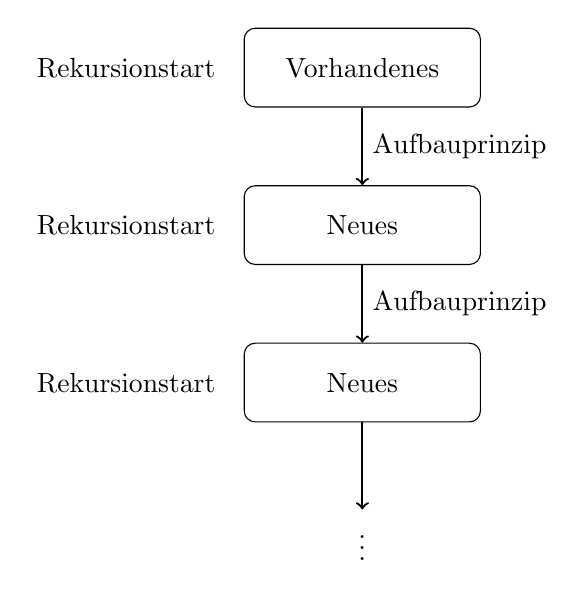
\begin{tikzpicture}[node distance = 2cm]
	\node (Vorhandenes) [rectangle, rounded corners, minimum width=3cm, minimum height=1cm, text centered, draw=black] {Vorhandenes};
	\node [anchor = west, left of = Vorhandenes, xshift = -1cm] {Rekursionstart};
	\node (Neues1) [rectangle, rounded corners, minimum width=3cm, minimum height=1cm, text centered, draw=black, below of = Vorhandenes] {Neues};
	\node [anchor = west, left of = Neues1, xshift = -1cm] {Rekursionstart};
	\node (Neues2) [rectangle, rounded corners, minimum width=3cm, minimum height=1cm, text centered, draw=black, below of = Neues1] {Neues};
	\node (dots) [below of = Neues2] {$\vdots$};
	\node [anchor = west, left of = Neues2, xshift = -1cm] {Rekursionstart};
	\draw [thick, ->] (Vorhandenes) -- node [anchor = west] {Aufbauprinzip} (Neues1);
	\draw [thick, ->] (Neues1) -- node [anchor = west] {Aufbauprinzip} (Neues2);
	\draw [thick, ->] (Neues2) -- (dots);
\end{tikzpicture}

Objekte:
\begin{itemize}
	\item Grundobjekte
		\begin{itemize}
			\item $ 0, 1, 2, ..., 100, ... $
			\item $ \N_0 $
		\end{itemize}
	\item Aufbauprinzipien
		\begin{itemize}
			\item Aufzählungsmenge zu angegebenen Elementen ist wieder ein Element\\
				Bsp.: $ \{1\} j$
			\item Regel: mathematisches Objekt, für das eine Elementaussage gilt\\
				$ A \cup B, A \cap B, A \setminus B, A \times B $
		\end{itemize}
\end{itemize}

Aussagen:
\begin{itemize}
	\item Grundaussagen:
		\begin{itemize}
			\item $ x = y $
			\item $ x, y $ mathematische Objekte
			\item $ x \in y $
		\end{itemize}
	\item Aufbauprinzip
		\begin{itemize}
			\item $ \iff $, $ \implies $, $ \wedge $, $ \vee $, $ \neg $, $ Q $ ($\forall$, $\exists$, $\exists!$), ``$ : $''
		\end{itemize}
\end{itemize}

\begin{definition}[Teilermenge]
	\label{def:Teilermenge}
	Es sei $ a \in \mathbb{N} $. Dann sei $ \mathcal{T}(n) $ die Menge aller positiven Teiler von $ a $, die größer als eins sind.
	\begin{example}
		\[ \mathcal{T}(5) = \{5\}, \mathcal{T}(6) = \{2, 3, 6\} \]
	\end{example}
	Bem.: $ \forall a \in \mathbb{N} : \mathcal{T}(a) \in \mathbb{N} $
\end{definition}

Wahrheiten:
\begin{itemize}
	\item Grundaxiome:
		\begin{itemize}
			\item $ 0 \in \N $
			\item $ 1 \in \N $
			\item $ x = x $ für definierte Objektausdrücke
		\end{itemize}
	\item Aufbauprinzip:
		\begin{itemize}
			\item Nachweisregeln,
			\item Benutzungsregeln
		\end{itemize}
\end{itemize}


%%%%%%%%%%%%%%%%%%%%%%%%%%%%
%%% Inklusion von Mengen %%%
%%%%%%%%%%%%%%%%%%%%%%%%%%%%

\section{Inklusion von Mengen}

\begin{example}
	Es sei $ X $ eine Menge $ A, B \subseteq X $ Teilmengen.\\
	Zeige $ A \cap B \subseteq A $.\\
	Zu zeigen $ \forall x \in ( A \cap B ) : x \in A $. Sei dazu $ x \in A \cap B $ gegeben. Zu zeigen: $ x \in A $. Da $ x \in A \cap B $ folgt (nach Definition zu ``$ \cap $ '')
	\[ x \in A \wedge x \in B \]
	Es gilt also insbesondere
	\[ x \in A, \qed \]
\end{example}

\begin{important}
	Man benutzt statt
	\[ \subseteq \]
	auch oft
	\[ \subset \]
	oder seltener
	\[ \subseteqq \]
	\[ A \subsetneqq B \iff A \subseteq B \wedge A \neq B \]
\end{important}

(\fbox{B.2}):\\
Sind $U, V $ Aussagen\\
Will man 
\[ U \iff V \text{zeigen, so ist es äquivalent dazu}\]
\[ ( U \implies V ) \wedge ( V \implies U ) \]
zu zeigen.\par

(\fbox{B.12}):\\
Um für Mengen $ C, D $ die Gleichheit $ C = D $ zu zeigen, zeigt man $ C \subseteq D \wedge D \subseteq C $\par

\[ A = B \iff A \subseteq B \wedge B \subseteq A \]

\begin{task}
	\label{task:16.1}
	Es seien $ X $ Menge und $A, B \subseteq X $ zwei Teilmengen.\\
	Beweisen Sie folgende Äquivalenz
	\[ A \cup B = X \text{ und } A \cap B \neq \emptyset \iff A = X \setminus B \]
\end{task}
\begin{proof}[to Task \ref{task:16.1}]
	Wir beweisen die Äquivalenz durch Beweis der beide Implikationen ``$ \implies $'' und ``$ \impliedby $''.\par
	\begin{description}
		\item[``$ \implies $'':]
		Wir nehmen an, dass
		\[ A \cup B = X \wedge A \cap B = \emptyset \]
		gilt
		z.z.: $ A = X \setminus B $.\\
		Dazu genügt es, die Inklusion
		\[ \underbrace{A \subseteq X \setminus B}_{\text{1.}} \wedge \underbrace{X \setminus B \subseteq A}_{\text{2.}} \]
		z.z.
		\begin{enumerate}[label=\arabic*.]
			\item \label{enum:ASubseteqXSetminusB} Wir zeigen $ A \subseteq X \setminus B $\\
				Es  sei $ x \in A $. z.z $ x \in X \setminus B $\\
				Da $ A \subseteq X $ gilt, $ x \in X $.\\
				Es bleibt z.z., dass 
				\[ x \notin B \]
				Wir führen einen Widerspruchsbeweis und nehmen dazu an, dass $ x \in B $ gilt. Dann folt aber $ a \in A \wedge x \in B $, also $ x \in A \cap B $. Wiederspruch, da $ A \cap B = \emptyset $\\
				Also muss $ x \notin B $ gelten. Insgesamt folgt
				\[x \in X \setminus B \]
				Da $ x \in A $ beliebig war, ist somit $ A \subseteq X \setminus B $ bewiesen.
			\item \label{enum:XSetminusBSubseteqA}Wir zeigen $ X \setminus B \subseteq A $. Sei $ x \in X \setminus B $. Dann gilt
				\[ x \in X \wedge x \notin B \]
				Da $ X = A \cup B $, folgt $ x \in A \vee x \in B $. Da aber
				\[ x \notin B \text{, folgt } x \in A \]
				Da $ x \in X \setminus B $ beliebig war, ist $ X \setminus B \subseteq A $ bewiesen.
		\end{enumerate}
		Damit (mit \ref{enum:ASubseteqXSetminusB} und \ref{enum:XSetminusBSubseteqA}) ist die Gleichheit $ A = X \setminus B $ bewiesen.

		\item[``$ \impliedby $'':]
			Wir nehmen an, dass $ A = X \setminus B $ gilt.\\
			z.z.: Es gilt $ \underbrace{ A \cup B = X }_{ I } $ und $ \underbrace{ A \cap B = \emptyset }_{ II } $\\
			Zum Beweis von $ I $ zeigen wir
			\begin{enumerate}
				\item \label{enum:ACupBSubseteqX} $ A \cup B \subseteq X $
				\item \label{enum:XSubseteqACupB} $ X \subseteq A \cup B $
			\end{enumerate}
			1. Zeige $ A \cup B \subseteq X $. Sei $ x \in A \cup B $. DAnn gilt $ ( x \in A ) \vee ( x \in B ) $. Gilt $ x \in A $, so folgt wegen $ A \subseteq X $ sofort $ x \in X $. Gilt $ x \in B $, so folgt wegen $ B \subseteq X $ sofort $ x \in X $. In beiden Fällen folgt also $ x \in X $, wie gewünscht.\par
			2. Zeige $ X \subseteq A \cup B $: Sei $ x \in X $.\\
			z.z.: $ x \in A \vee x \in B $\\
			1. Fall: $ x \in A \implies x \in A \vee x \in B $\\
			2. Fall: $ x \notin A $ z.z. $ x \in B $\\
			(Annahme von $ x \notin B $. Dann gilt
			\[ x \in X \setminus B \]
			Da aber $ X \setminus B = A $ folgt $ x \in A $, was zu einem Wiederspruch führt.\\
			Also muss $x  \in B $ gelten.)
			Da $ A = X \setminus B $ folgt
			\[ x \notin X \setminus B \]
			Also gilt
			\[ \neg ( x \in X \wedge x \notin B ) \]
			\[ x \notin X \vee x \in B \]
			Fall 1: $ x \notin X $ Wiederspruch zur Vor. $ x \in X $, also muss
			Fall 2: 
			\[x \in B \]
			gelten.\par
			Insgesamt $ x \in A \cup B $, wie gewünscht
	\end{description}
\end{proof}

\begin{lemma}
	Es sei $ a \in \mathbb{N} $. Dann gilt
	\begin{enumerate}[label=(\roman*)]
		\item $ a \in \mathcal{T}(a) $ \label{enum:one}
		\item $ \mathcal{T}(a) \neq \emptyset $ \label{enum:two}
	\end{enumerate}
	\begin{proof}
		Es sei $ a \in \N $ Es gilt $ a \mid a $, denn $ a = 1 \times a $, also $ \exists c \in \N : (a = c \times a ) $, nämlich $ c \coloneqq 1 $.\\
		Da $ a \mid a $ gilt und $ a > 1 $ ist, folgt sofort (nach Definition \ref{def:Teilermenge}) $ a \in \mathcal{T}(a) $. Dies beweist \ref{enum:one}.
		Da nach \ref{enum:one} gilt, dass $ a \in \mathcal{T}(a) $ folgt sofort $ \mathcal{T}(a) \neq \emptyset $. Was \ref{enum:two} beweist.
	\end{proof}
\end{lemma}

\begin{corollary}
	Es sei $ a \in \N $, $ a > 1 $.\\
	Da $ \mathcal{T}(a) $ eine nicht leere Teilmenge von $ \N $ ist, hat $ \mathcal{T}(a) $ ein kleinstes Element
\end{corollary}

\begin{theorem}
	\label{theorem:ExistsPrimeFactor}
	Es sei $ a \in \N $, $ a > 1 $\\
	Dann gibt es eine Primzahl $ p \in \mathbb{P} $ mit $ p \mid a $
	\[ \forall a \in \N_{>1} : \exists p \in \mathbb{P} : p \mid a \]
	\begin{proof}
		Es sei $ a \in \N_{>1} $ beliebig.\\
		zu zeigen: $ \exists p \in \mathbb{P} : p \mid a $\\
		Betrachten $ \mathcal{T}(a) $. Diese hat ein kleinstes Element. Nennen wir dieses $ \beta $.\par
		Beh.: $ \beta \in \mathbb{P} $.\\
		Wir führen einen Widerspruchsbeweis und nehmen an, dass $ \beta \notin \mathbb{P} $. Dann hat $ \beta $ einen Teiler $ q \in \N $ mit
		\[ 1 < q < \beta. \]
		Da $ q \mid \beta $  und $ \beta \mid a $, folgt nach Teilbarkeitsregeln $ q \mid a $. Also (beachte $ q > 1 $) $ q \in \mathcal{T} $.\\
		Widerspruch, da $ q < \beta $ und $ \beta $ das kleinste Element von $ \mathcal{T}(a) $ ist.
		somit muss
		\[ \beta \in \mathbb{P} \qed \]
	\end{proof}
\end{theorem}

\begin{theorem}[(Euklid)]
	Es gibt unendlich viele Primzahlen
	\begin{proof}[Widerspruchsbeweis]
		Wir nehmen dazu an, dass es nur endlich viele Primzahlen gibt. Sagen wir
		\[ p_1, p_2, ..., p_n \quad \text{(d.h. $ \mathbb{P} = \{ p_1, p_2, ... p_n \} $)} \]
		Wir betrachten
		\[ a \coloneqq p_1 \times p_2 \times ... \times p_n + 1 \]
		Es gilt $ a \in \N $, $ a > 1 $. Somit (nach vorigem Satz \ref{theorem:ExistsPrimeFactor}) existiert $ p \in \mathbb{P} $ mit $ p \mid a $. Also gilt $ p \in \{ p_1, p_2, ..., p_n \} $\\
		Also folgt $ p \mid ( p_1 \times p_2 \times ... \times p_n ) $\\
		Somit folt (beachte $ p \mid a $)
		\[ p \mid ( \underbrace{ a - p_1 \times p_2 \times ... \times p_n ) }_{=1} \]
		Also $ p \mid 1 $ $ \implies $ Widerspruch: Also war unsere Annahme falsch und es muss unendlich vile Primzahlen geben \qed
	\end{proof}
\end{theorem}

\section{Vollständige Induktion}

\begin{theorem}[Vollständige Induktion]
	\label{theo:Induktion}
	Sei $ A(n) $ eine Eigenschaft für natürliche Zahlen\\
	Es gelte
	\begin{enumerate}[label=(\roman*)]
		\item $ A(1) $, d.h. $ 1 $ hat diese Eigenschaft
		\item $ \forall a \in \N : A(n) \implies A(n+1) $
	\end{enumerate}
	d.h. für alle $ n \in \N $ gilt: Wenn $ n $ die Eigenschaft hat, dann hat $ n + 1 $ die Eigenschaft.
	Dann gilt $ A(n) $ für \underline{alle} $ n \in \N $
	\begin{blackbox}[Induktionsanfang (I.A.)]
		$ A(1) $ überprüfen auf Wahrheitswert (muss wahr sein)
	\end{blackbox}
	\begin{blackbox}[Induktionsschritt (I.S.)]
		Es sei $ n \in N $
		\[ \underbrace{A(n)}_{\text{Induktionsvoraussetzung (I.V.)}} \implies A(n+1) \]
	\end{blackbox}
\end{theorem}

\begin{task}
	Zeigen Sie mithilfe volllständiger Induktion, dass für all $n \in \N $ gilt:
	\[ 7 \mid \left( 5^{2 \cdot n} - 2^{2 \cdot n} \right) \qquad A(n) \]
	\begin{proof}
		\begin{description}
			\item[I.A. ($n = 1$)] Z.z.: $ 7 \mid \left( 5^{2 \cdot 1} - 2^{2 \cdot 1} \right) $\\
				Da $ 5^2 - 2^2 = 21 = 7 \cdot 3 $, also folgt $ 7 \mid \left( 5^{2 \cdot 1} - 2^{2 \cdot 1} \right) $
			\item[I.S.] Es sei $ n \in \N $
				\begin{description}
					\item[I.V.] \label{Ind.1:I.V.} Es gelte $ A(n) $ d.h. wir nehmen an, dass
						\[ 7 \mid \left( 5^{2n} - 2^{2n} \right) \]
				\end{description}
				z.z.: (I. Behauptung) $ A( n + 1 ) $ gilt,\\
				d.h.: $ 7 \mid \left[ 5^{2 \cdot ( n + 1 )} - 2^{2 \cdot ( n + 1 )} \right] $\\
				Es gilt
				\begin{align*}
					5^{2 \cdot ( n + 1 )} - 2^{2 \cdot ( n + 1 )} &= 5^{2n + 2} - 2^{2n + 2}\\
						~&= 25 \cdot 5^{2n} - 4 \cdot 2^{2n}\\
						~&= 25 \cdot 5^{2n} - 25 \cdot 2^{2n} + 25 \cdot 2^{2n} - 4 \cdot 2^{2n}\\
						~&= 25 \cdot \left( 5^{2n} - 2^{2n} \right) + ( 25 - 4 ) \cdot 2^{2n}\\
				\end{align*}
				Da nach \ref{Ind.1:I.V.} die Teilbarkeit
				\[ 7 \mid \left( 5^{2n} - 2^{2n} \right) \]
				gilt und auch $ 7 \mid (25 - 4) $ gilt, folgt (Teilbarkeitsregeln !) $ 7 \mid \left( 5^{2 \cdot ( n + 1 )} - 2^{2 \cdot ( n + 1 )} \right) $, \qed
		\end{description}
		Mit Induktionsprinzip ergibt insgesamt
		\[ \forall n \in \N : 7 \mid \left( 5^{2n} - 2^{2n} \right) \]
	\end{proof}
\end{task}

\begin{definition}
	Wir wollen die Behauptung beweisen:
	\[ \forall n \in \N : A(n) \]\par
	Teil 1: I.A.\\
	Wir beweisen, dass $ A(1) $ gilt\par
	Tail 2: I.S.\\
	von $ n $ nach $ n + 1 $
	\begin{description}
		\item[I.V.:] Es gelte $ A(n) $ für $ n \in \N $\\
			Z.z.: Es gilt auch $ A( n + 1 ) $
			\[ \implies \forall n \in \N : A(n) \]
	\end{description}
\end{definition}

\begin{task}
	\begin{proof}[$ \forall n \in \N : \sum_{k = 1}^{n}\left( 2k - 1 \right) = n^2 $]
		\begin{description}
			\item[I.A. ($ n = 1 $)]\label{proof:1:des:I.A.}~\\
				z.z.: $ \sum_{k = 1}^{1}\left( 2k - 1 \right) = 1^2 $\\
				Es gilt
				\[ \sum_{k = 1}^{1}\left( 2k - 1 \right) = 2 \cdot 1 - 1 = 1 \]
				und
				\[ 1^2 = 1 \]
				was \ref{proof:1:des:I.A.} beweist
			\item[I.S.] z.z. (I. Beh.)
				\[ \sum_{k = 1}^{n + 1}\left( 2k - 1 \right) = ( n + 1)^2 \]
				\begin{description}
					\item[I.V.] \label{proof:1:des:I.V.} Es sei $ n \in \N $, es gelte
						\[ \sum_{k=1}^{n}\left( 2k - 1 \right) = n^2 \]
				\end{description}
				\[ \sum_{k = 1}^{n + 1}\left( 2k - 1 \right) = \underbrace{\sum_{k = 1}^{n}\left( 2k - 1\right)}_{\text{ersten $ n $ Summanden}} + \underbrace{\left( 2( n + 1 ) - 1 \right)}_{\text{ $n + 1 $-ter Summand}} \]
				\begin{align*}
					\sum_{k = 1}^{n + 1}\left( 2k - 1 \right) &= n^2 + \left( 2 ( n + 1 ) - 1 \right)\\
						~&= n^2 + 2n + 2 - 1\\
						~&= n^2 + 2n + 2\\
						~&= ( n + 1 )^2, \qed
				\end{align*}
		\end{description}
		Mit dem Prinzip der vollständigen Induktion könnnen wir folgern, dass gilt
		\[ \forall n \in \N : \sum_{k = 1}^{n} = n^2 .\]
	\end{proof}
\end{task}

In reiner Zahlentheorie betrachtete man die Induktion als Axiom
\begin{axiom}[Induktionsaxiom]
	Es sei $ M \subseteq \N $ eine teilmenge mit
	\begin{enumerate}[label=(\roman*)]
		\item $ 1 \in M $
		\item $ \forall n \in \N : n \in M \implies n + 1 \in M $
	\end{enumerate}
	Dann ist
	\[ M = \N \]\par
	Dieses Axiom ermöglicht das Beweisverfahren durch vollständige Induktion, denn:\\
	Es sei $  M \coloneqq \{ n \in \N : A(n) \} $, Gilt
	\begin{enumerate}[label=(\roman*)]
		\item $ 1 \in M $, d.h. es gilt $ A(1) $
		\item $ \forall n \in \N : Wenn n \in M $ 8also $ A(n) $ gilt), folgt $ n + 1 \in M $ (also $ A( n + 1 ) $ gilt)
	\end{enumerate}
	Dann folgt nach Axiom
	\[ M = \N \]
	d.h. $ \forall n \in \N : A(n) $
\end{axiom}

\section{Abbildung (Funktionen)}

\begin{definition}
	Es seien $ X, Y $ bel. Mengen.\\
	Eine \underline{Abbildung} (oder Funktion) $ f $ von $ X $ nach $ Y $ ist eine Vorschrift, die jedem Element $ x \in X $ genau ein Element $ y_x \in Y $ zuordnet.
	\[ f :
		\begin{cases}
			X \to Y\\
			x \mapsto y_x
		\end{cases}
		f \text{ ist Abbildung von $ X $ nach $ Y $, $ x $ wird auf $ y_x $ abgeblidet}
	\]
	Das dem Element $ x \in X $ in eindutiger Weise durch $ f $ zugeordnete Element $ y_x $ wird auch mit \[ f(x) \] bezeichnet; $ f(x) $ \underline{heißt das Bild von $ x $ unter $ f(x) $}, oder \underline{der Wert von $ f $ an der Stelle $ x $}.
	\[ X \text{heißt auch \underline{Definitionsbereich von $ f $}, (Auch $ \operatorname{Def}(f) $)} \]
	\[ Y \text{ heißt auch \underline{Zielbereich von} $ f $ und} \]
	\[ W_f \coloneqq \{ y \in Y : \exists x \in X : f(x) = y \} \]
	der (exakte) \underline{Wertebereich von} $ f $ oder kurz das \underline{Bild von} $ f $. Andere Bezeichnungen für $ W_f : \operatorname{Bild}(f) \text{ oder } f(X) $\par
	\begin{definition}
		Ein $ x \in X $ heißt Urbild von $ y \in Y $, falls $ f(x) = y $ gilt.
		\begin{example}
			$ X, Y \in \R $. Betrachte \[ f: \begin{cases} \R \to \R\\ x \mapsto x^2 \end{cases} \] $ \operatorname{Def}(f) = \R $, Zielbereich von $ \R $; $ \operatorname{Bild}(f) = f(\R) = \R_{\geq 0} = \R^{+} $
		\end{example}
		\begin{example}[keine Funktion $ f: \R \to \R, x \mapsto \begin{cases} ( x - 1 ), & \text{falls } x \geq 1\\ x + 2, & \text{falls } x \leq 1 \end{cases} $]
			\begin{itemize}
				\item Urbilder von $ 4 $ unter $ f : \text{ für welche $ x \in \R $ gilt $f(x) = 4 $? $ : 2, -2 $} $
				\item Urbilder von $ -2 \in \R = Y $ unter $ f $? Für welche $ x \in \R $ gilt $ f(x) = -2 $? d.h. $ x^2 = -2 \contradiction $ kein $ x \in \R $
				\item Urbilder von $ i $ unter $ f $? $ \contradiction $ kann man nicht fragen. $ i \notin \R $
			\end{itemize}
		\end{example}
	\end{definition}
\end{definition}

\begin{definition}[Graph]
	Ist $ f : X \to Y $ eine Abbildung, dann heißt
	\[ \operatorname{Graph}(f) \coloneqq \{ ( x, y ) \in X \times Y \mid y = f(x) \]
	der \underline{Graph von $ f $}.
	\begin{example}
		\begin{math}
			g : X = \{ 1, 2, 3 \} \to \{ -2 , -1, 0, 1, 2 \} = Y,%
			\begin{cases}
				1 \mapsto 1\\
				2 \mapsto 2\\
				3 \mapsto 0
			\end{cases}
		\end{math}\\
		$ \operatorname{Def}(g) = \{ 1, 2, 3 \} $, $ \operatorname{Bild}(g) = g(X) = \{ 1, 2, 0 \} $
		\begin{itemize}
			\item Urbilder von $ 0 $: $ 3 $
			\item Urbilder von $ - 2 $: keine
		\end{itemize}
		\begin{align*}
			g^{-1}(\{ 0, 2 \}) \coloneqq &\{ x \in \{ 1, 2, 3 \} : ( g(x) = 0 ) \vee ( g(x) = 2 )\}\\
			= &\{ x \in \{ 1, 2, 3 \} : g(x) \in \{ 0, 2 \} \}
		\end{align*}
		\[ g(\{ 1, 3 \}) \coloneqq \{ g(x) : x \in \{ 1, 3 \} \} = \{ g(1), g(3) \} = \{ 1, 0 \} \]
	\end{example}
\end{definition}

\begin{definition}
	Es sei $ f : X \to Y $ eine Abbildung
	\begin{itemize}
		\item[\circled{1}] Für eine Teilmenge $ A \subseteq X $ heißt
			\begin{align*}
				f(A) \coloneq &\{ f(x) \mid x \in A \} \subseteq Y\\
				= &\{ y \in Y \mid \exists x \in A : f(x) = y \}
			\end{align*}
			\underline{Bild der Menge $ A $ unter $ f $}.
		\item[\circled{2}] Für eine Teilmenge $ B \subseteq Y $ heißt die Menge
			\[ f^{-1}(B) = \{ x \in X : f(x) \in B \} = \{ x \in X : \exists y \in B : f(x) = y \} \]
			das \underline{Urbild von $ B $ unter $ f $}\par
			Falls $ B = \{ y \} $\\
			Für $ y \in Y $ ist das Urbild von $ y $ unter $ f $ die Menge
			\[ f^{-1}(y) \coloneqq \{ x \in X : f(x) \in \{ y \} = \{ x \in X : f(x) = y \} \]
	\end{itemize}
\end{definition}

\begin{example}[$
	f :
	\begin{cases}
		\R \to \R\\
		x \to x^2
	\end{cases}
	$]
	$ f([ 0, 1 ]) = \{ x^2 : x \in [ 0, 1 ] \} \overset{!?}{=} [ 0, 1 ] $\\
	$ f(\{ 0, 2 \} ) = \{ f(0), f(2) \} = \{ 0, 4 \} $\\
	$ \operatorname{Bild}(f) = f(\R) = \R_{\geq0} $\par
	$ f^{-1}([-1, 1]) = \{ x \in \R : f(x) \in [-1, 1]\} \overset{?!}{=} [-1, 1] $\\
	$ f^{-1}(\{0, 1\}) = \{ x \in \R : f(x) \in \{0, 1\} \} = \{ x \in \R : f(x) = 0 \vee f(x) = 1 \} = \{ 0, 1, -1 \} $
\end{example}

\section{Grobe Einteilung von mathematischen Objekten}
\begin{tabularx}{\textwidth}{>{\raggedright}X>{\raggedright}X>{\raggedright}X}
	\multicolumn{1}{c}{Zahlen} & \multicolumn{1}{c}{\mynode{Mengen}{Mengen}} & \multicolumn{1}{c}{\mynode{Funktionen}{Funktionen}}\\\hline
	\begin{itemize}
		\item \raggedright Ausgangsmaterial zur Ob\-jektbildung
	\end{itemize} &
	\begin{itemize}
		\item schaffen Begriffe
		\item[] ``gerade Zahlen''
		\item[] $ \quad \vdots $
		\item dienen der Zusammenfassung/Einteilung von Objekten
	\end{itemize} &
	\begin{itemize}
		\item schaffen
		\item[] \underline{\mynode{Zusammenhänge}{Zusammenhänge}}
	\end{itemize}
\end{tabularx}\\
Was macht man damit\mynode{?}{?}
\begin{itemize}
	\item abhängige (Mess-)Werte
\end{itemize}
\begin{tikzpicture}[remember picture, overlay]
	\draw[->] ([xshift=2pt]Mengen.east) to ([xshift=-2pt]Funktionen.west);
	\draw[->,>=stealth] ([yshift=-2pt]Zusammenhänge.south) to [out=-90, in = 0] ([xshift=2pt]?.east);
\end{tikzpicture}

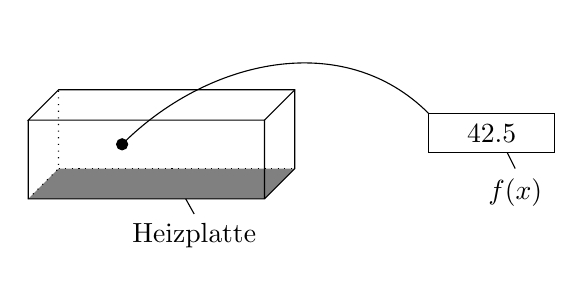
\begin{tikzpicture}
	\fill[gray] ( 0, 0, 0 ) -- ( 3, 0, 0 ) -- ( 3, 0, 1 ) -- ( 0, 0, 1 );
	\draw ( 0, 1, 1 ) -- ( 0, 0, 1 ) -- ( 3, 0, 1 ) -- ( 3, 1, 1 ) -- ( 0, 1, 1 ) -- ( 0, 1, 0 ) -- ( 3, 1, 0 ) -- ( 3, 0, 0 ) -- ( 3, 0, 1 );
	\draw[dotted] ( 0, 0, 1 ) -- ( 0, 0, 0 ) -- ( 0, 1, 0 );
	\draw[dotted] ( 0, 0, 0 ) -- ( 3, 0, 0 );
	\draw ( 3, 1, 0 ) -- ( 3, 1, 1 );
	\draw[fill] ( 1, 0.5, 0.5 ) circle (2pt);
	\draw ( 4.7, 0.2, 0 ) rectangle ( 6.3, 0.7, 0 );
	\node [anchor = center ] at ( 5.5, 0.45, 0 ) {$\qty{42.5}{\celsius}$};
	\draw[-,>=stealth] ( 1, 0.5, 0.5 ) to [out = 45, in = 135] ( 4.7, 0.7, 0 );
	\draw ( 2, 0, 1 ) -- ( 2.3, 0, 1.5 ) node[anchor = north] {Heizplatte};
	\draw ( 5.7, 0.2, 0 ) -- ( 5.8, 0.0, 0 ) node[anchor = north] {$ f(x) $};
\end{tikzpicture}

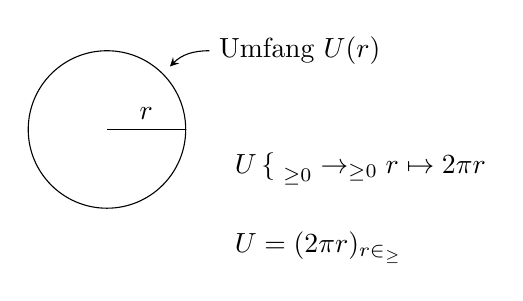
\begin{tikzpicture}
	\draw ( 0, 0 ) circle (1);
	\draw ( 0, 0 ) -- node [anchor = south] {$r$} ( 1, 0 );
	\draw[->, > = stealth] ( 1.3, 1 ) node [anchor = west] {Umfang $U(r)$} to [out = 180, in = 45] ( 0.8, 0.8 );
	\node [anchor = west] at ( 1.5, -0.5 ) {$ U \coloneqq \begin{cases} \R_{\geq 0} \to \R_{\geq 0}\\r \mapsto 2 \pi r \end{cases}$};
		\node [anchor = west] at ( 1.5, -1.5 ) {$ U = (2 \pi r )_{r \in \R_{\geq}} $};
\end{tikzpicture}

Rezept/Bastelanleitung\\
Zutat $ x $ mit $ x \in X $\\
Ergebnis: z.B. $ 2 \pi x $

\begingroup
	\setlength\tabcolsep{0pt}
	\begin{tabularx}{0.9\textwidth}{l>{\ }X}
		Funktionsausdruck $ \hat= $ &allg. Situationsbeschreibung mit einer Ergebnisdefinition\\
		~&Bennenung/Indizierung\\
		~&\quad``Abzählen''. Jedes Objekt bekmomt eine Nummer bzw. Jede Nummer bekommt ein Objekt\\
	\end{tabularx}
\endgroup

$ f \coloneqq ( \N, \Z, \Q, \R, \dotsc) $ \underline{Tupel} sind \underline{Funktionen}\\
$ \quad \operatorname{Def}(f) = \{ 1, 2, 3, \dotsc, n \} \quad f(1) = \N \text{ oft } f_1 $\\
$ \operatorname{Bild}(f) = \{ y \in U: \exists x \in \operatorname{Def}(f) : y = f(x) \} = \{ \N, \Z, \Q, \R, \dotsc \} $

\begin{itemize}
	\item Attribute von Objekten\\[1em]
		\begin{tabular}{c|c}
			Land & Hauptstadt\\
			\hline
			D	& Berlin\\
			CH	& ?\\
			F	& Paris\\
			A	& Wien\\
		\end{tabular}
		\hspace{2em}
		\begin{minipage}{0.5\textwidth}
			Tabellen! c:\\
			``$\operatorname{Hauptstadt}(\operatorname{Land})$''
		\end{minipage}
\end{itemize}

\hrule width 50pt \kern 1pt \hrule width 50pt
Was macht man damit ...?
\begin{itemize}
	\item abhängige (Mess-)Werte \qquad $ (2 \pi r )_{ r \in \R_{\geq} } $
	\item Benennung/Indizierung \qquad $ ( \N, \Z, \Q, \R ), ( 2i - 1 )_{ i \in \N } = \{ 2i - 1 : i \in \N \} $
	\item Attribute von Objekten
\end{itemize}

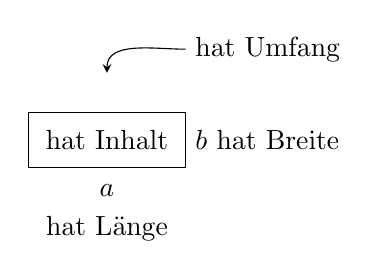
\begin{tikzpicture}
	\draw ( 0, 0 ) rectangle node {hat Inhalt} ( 2, 0.7 );
	\node [anchor = north] at ( 1, -0.5 ) {hat Länge};
	\node [anchor = north] at ( 1, -0.1 ) {$a$};
	\node [anchor = west] at  ( 2, 0.35 ) {$ b $ hat Breite};
	\draw[->, > = stealth] ( 2, 1.5 ) node [anchor = west] {hat Umfang} to [out = 180, in = 90] ( 1, 1.2 );
\end{tikzpicture}
\hspace{2em}
\begin{minipage}{0.5\textwidth}
	$ R \coloneqq \R_{>0}^{2} $ \qquad $ ( \Z, + ) $\\
	Länge $ \coloneqq (r_1)_{r \in R} $\\
	Breite $ \coloneqq ( r_2 )_{r \in R} $\\
	Umfang $ \coloneqq ( 2r_1 + 2r_2)_{r \in R} $\\
	Inhalt $ \coloneqq ( r_1, r_2 )_{r \in R} $
\end{minipage}

\begin{example}[``Gleichungen'']
	Finde $ x \in \R $, sodass gilt
	\begin{enumerate}[label=\alph*)]
		\item $ x^3 + x = 1 $ \quad\qquad x-Abhängigkeit durch Funktion $ f : (x^3 + x )_{x \in \R} $
		\item $ x^3 + x =  -5 $ \qquad beschreibe rechte Seite jeweils durch ein Element $ y \coloneqq 1 $
	\end{enumerate}
	$ ( f, y ) $ kodiert die Gleichung
\end{example}

\begin{definition}
	Unter einer Gleichung verstehen wir ein Paar $ (f, y ) $ mit einer Funktion $ f $ und einem Element $ y $.\\
	Die Lösungsmenge einer Gleichung $ (f, y ) $ ist gegeben durch $ \operatorname{L"os}(f, y)\bigl(=\operatorname{L"os}(f, y)\bigr) = \{x \in \operatorname{Def}(f) : f(x) = y \} $\\
	Gleichungen = $ \mathcal{F} \times \mathcal{U}  ( \mathcal{F} \coloneqq \text{ alle Funktionen }, \mathcal{U} \coloneqq \text{ alle Elemente } ) $

	\begin{tabularx}{\textwidth}{XcX}
		Eigenschaften von Gleichungen & \;\; ergeben sich \;\; & Eigenschaften der zugehörigen Funktion\\\toprule
		``Lösbarkeit'' für alle rechte Seiten aus einer Menge $ W $ &~& ``$ f $ ist \underline{surjektiv nach W}'' ($ f $ nimmt alle Werte von $ W $ an)\\
		$ \forall y \in W : \exists x \in \operatorname{L"os}(f, y) $ & $ \iff $ & $ \forall y \in W : \exists x \in \operatorname{Def}(f) : f(x) = y $\\
		\midrule
		``Eindeutigkeit von Lösungen'' &~& ``$ f $ ist \underline{injektiv}'' ($ f $ nimmt keinen Wert mehrfach an)\\
		$ \forall y \in \operatorname{Bild}(f) : \exists! x \in \operatorname{L"os}(f, y) $ & $ \impliedby $ & $ \neq \exists u,v \in \operatorname{Def}(f) : u \neq v \wedge f(u) = f(v) $\\
		``Existenz und Eindeutigkeit'' von Lösungen zu $ ( f, y ) $ für $ f : A \to B $ und alle $ y \in B $ &~& ``$ f $ ist \underline{bijektiv} von $ A $ nach $ B $, d.h. $ f : A \to B $ injektiv und $ f : $ surjektiv nach $ B $
	\end{tabularx}
\end{definition}

\begin{example}[$ f \coloneqq (x^2)_{x \in \Q} \quad g \coloneqq (x^2)_{x \in \R}$]
	$ f, g $ surjektiv nach $ \Q $?: nein\\
	$ f, g $ surjektiv nach $ \Q_{\geq 0} $?: für $ g $: ja, für $ f $: nein\\
	$ f, g $ injektiv: nein $ f(1) = g(1) = g(-1) = f(-1) $\\
	$ f = ( x^3 + x )_{x \in \R} \quad f^{\prime} = ( x^2 + 1 )_{x \in \R} \implies f^{\prime} \geq 1 > 0 \implies f \text{ streng monoton wachsend} $\\
	alle Gleichungen zu $ f $ mit $ y \in \R $ sind eindeutig lösbar
	\[ f \text{ ist bijektiv von $ \R $ nach $ \R $} \]
	$ \exists a \in \R : \operatorname{L"os}(f, y) = \{ a \} $
	$ \operatorname{Eintrag}(\{ a \}) = a \quad \operatorname{Eintrag}(\operatorname{L"os}(f, 1)) = $ ist \underline{die} Lösung von $ (f, 1) $ ``$ x^3 + x = 1 $''\\[2pt]
	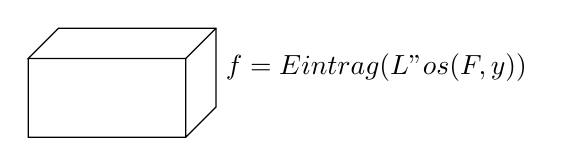
\begin{tikzpicture}
		\draw ( 0, 1, 1 ) -- ( 0, 0, 1 ) -- ( 2, 0, 1 ) -- ( 2, 1, 1 ) -- ( 0, 1, 1 ) -- ( 0, 1, 0 ) -- ( 2, 1, 0 ) -- node [anchor = west] {$ f = \operatorname{Eintrag}(\operatorname{L"os}( F, y)) $} ( 2, 0, 0 ) -- ( 2, 0, 1 );
		\draw ( 2, 1, 1 ) -- ( 2, 1, 0 );
	\end{tikzpicture}
\end{example}

\begin{theorem}
	\begin{tabularx}{\textwidth}{l>{\ }X}
		\setlength\tabcolsep{0pt}
		Es seien $ f : X \to Y $ eine Abbildung & und $ A_1, A_2 $ Teilmengen von $ X $ (d.h. $ A_1 \subseteq X, A_2 \subseteq X $)\\
		~& sowie $ B, B_1, B_2 $ Teilmengen von $ Y $ (d.h. $ B, \subseteq Y, B_1 \subseteq Y, B_2 \subseteq Y $)\\
	\end{tabularx}\\
	Dann gelten folgende Aussgaen:
	\begin{enumerate}[label=(\arabic*)]
		\item $ A_1 \subseteq A_2 \implies f(A_1) {\color{yellow} \subseteq} f(A_2) $\\
			$ B_1 \subseteq B_2 \implies f^{-1}(B_1) { \color{yellow} \subseteq } f^{-1}(B_2) $\\
			d.h. sowohl ``Bild als auch Urbild'' respektieren die Inklusion
		\item \label{enum:2023-10-21-01-53}$ f(A_1 \cup A_2) = f(A_1) \cup f(A_2) = \{ f(a) : a \in A_1 \cup A_2 \} $\\
			$ f(A_1 \cap A_2) \subseteq f(A_1) \cap f(A_2) $
		\item $ f^{-1}(B_1 \cup B_2) = f^{-1}(B_1) \cup f^{-1}(B_2) $\\
			$ f^{-1}(B_1 \cap B_2) = f^{-1}(B_1) \cap f^{-1}(B_2) $\\
	\end{enumerate}
\end{theorem}
Zum Beweis der ersten Aussage in \ref{enum:2023-10-21-01-53} zeigen wir
\[ I f(A_1 \cup A_2) \subseteq f(A_1) \cup f(A_2) \]
\[ II f(A_1) \cup f(A_2) \subseteq f(A_1 \cup A_2) \]
\par
\begin{description}
	\item[I.] Sei $ y \in f(A_1 \cup A_2) $. Z.z.: $ y \in f(A_1) \wedge f(A_2) $\\
		Da $ y \in f(A_1 \cup A_2) $, existiert ein 
		\[ a \in A_1 \cup A_2 \text{ (d.h. $ a \in A_1 \wedge A_2 $)} \]
		mit
		\[ f(a) = y. \]
		\begin{description}
			\item[1. Fall:] ($ a \in A_1 $).\quad Dann existiert also $ a \in A_1 $ mit $ f(a) = y $, also
				\[ y \in f(A_1) \]
			\item[2. Fall:] ($ a \in A_2 $).\quad Dann existiert also $ a \in A_2 $ mit $ f(a) = y $, also
				\[ y \in f(A_2) \]
		\end{description}
		Insgesamt folgt
		\[ y \in f(A_1) \vee y \in f(A_2), \qed \]
	\item[II.] Sei $y \in f(A_1) \cup f(A_2) $. Z.z.: $ y \in f(A_1 \cup A_2) $\\
		Da $ y \in f(A_1) \cup f(A_2) $, folgt
			\[ y \in f(A_1) \vee f(A_2) \]
		\begin{description}
			\item[1. Fall:] $ y \in f(A_1) $. Dann existiert $ a \in A_1 $ mit
				\begin{equation}
					\label{eq:2023-10-21-02-13}
					y = f(a)
				\end{equation}
				Da $ A_1 \subseteq ( A_1 \cup A_2 ) $ folgt $ a \in ( A_1 \cup A_2 ) $, also (wegen \ref{eq:2023-10-21-02-13}) $ y \in f(A_1 \cup A_2) $
			\item[2. Fall:] $ y \in f(A_2) $. Dann existiert $ a \in A_2 $ mit
				\begin{equation}
					\label{eq:2023-10-21-02-13_2}
					y = f(a)
				\end{equation}
				Da $ A_2 \subseteq ( A_1 \cup A_2 ) $ folgt $ a \in ( A_1 \cup A_2 ) $, also (wegen \ref{eq:2023-10-21-02-13_2}) $ y \in f(A_1 \cup A_2) $
		\end{description}
\end{description}

\section{Verkettung von Funktionen}
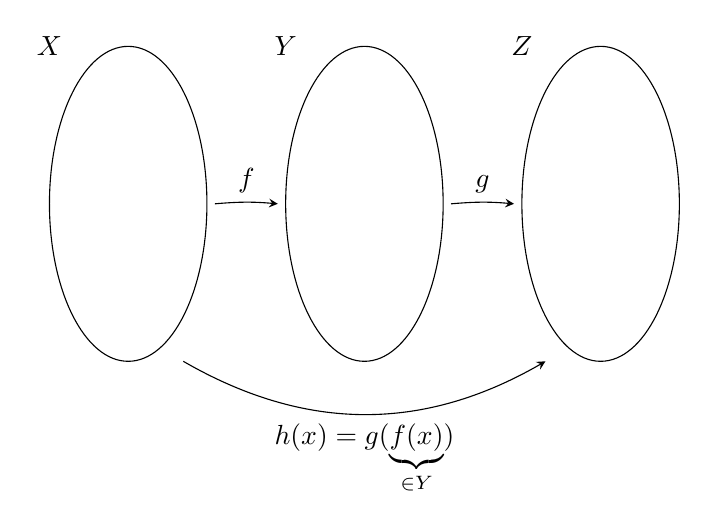
\begin{tikzpicture}
	\draw ( 0, 0) circle [x radius = 1, y radius = 2];
	\node at ( -1, 2 ) {$X$};
	\draw ( 3, 0) circle [x radius = 1, y radius = 2];
	\node at ( 2, 2 ) {$Y$};
	\draw ( 6, 0) circle [x radius = 1, y radius = 2];
	\node at ( 5, 2 ) {$Z$};
	\draw[->, > = stealth] ( 1.1, 0 ) to [out = 5, in = 175] node [anchor = south] {$ f $} ( 1.9, 0);
	\draw[->, > = stealth] ( 4.1, 0 ) to [out = 5, in = 175] node [anchor = south] {$ g $} ( 4.9, 0);
	\draw[->, > = stealth] ( 0.7, -2 ) to [out = -30, in = -150] node [anchor = north] {$ h(x) = g(\underbrace{f(x)}_{\in Y}) $} ( 5.3, -2 );
\end{tikzpicture}
\begin{definition}
	Die \underline{Identität auf $ X $} (identische Abbildung auf $ X $) ist die Abbildung
	\[ \operatorname{id}_x : X \to X, x \mapsto x \]
	z.B. $ \operatorname{id}_{\R} : \R \to \R, x \mapsto x $\\
	$ \quad \operatorname{id}_{\{1, 2\}} : \{ 1, 2 \} \to \{ 1, 2 \}, 1 \mapsto 1, 2 \mapsto 2 $
\end{definition}

\begin{definition}
	Seien $ f : X \to Y_1, g : Y_2 \to Z $ zwei Abbildungen mit 
	\[ f(X) \subseteqq Y_2 \]
	Die \underline{Verkettung $ g \circ f $} (lies ``$ g $ nach $ f $'') ist die Abbildung
	\[ g \circ f : X \to Z, x \mapsto g(f(x)) \]
	d.h.
	\[ g \circ f \coloneqq g(f(x)) \quad \text{für alle $ x \in X $} \]
	! Zuerst wird $ f $ angewendet, dann $ g $. !
\end{definition}

\begin{example}
	$ f :
	\begin{cases}
		\R_{0}^{+} \to \R_{0}^{+}\\
		x \mapsto x^2
	\end{cases},
	g :
	\begin{cases}
		\R_{0}^{+} \to \R_{0}^{+}\\
		x \mapsto \sqrt{x}
	\end{cases} $
	Es können beide Verkettungen $ g \circ g $ und $ f \circ g $ gebilded werden. Für $ x \in \R_{0}^{+} $:
	\[ ( g \circ f )(x) = g(f(x)) = g(x^2) = \sqrt{x^2} = \mid x \mid = x \text{ da $ x \in \R_{0}^{+} $} \]
	\[ ( f \circ g )(x) = f(g(x)) = f(\sqrt{x}) = \sqrt{x}^2 = x \]
	\[ g \circ f = f \circ g = \operatorname{id}_{\R_0^+} \]
\end{example}

\begin{definition}
	$ f : X \to Y $ heißt bijektiv, wenn sie surjektiv und injektiv ist.
\end{definition}

\begin{theorem}
	Sei $ f : X \to Y $ eine Abbildung.
	\begin{enumerate}[label=(1\arabic*)]
		\item \label{enum:2023-10-21-03-17} Existiert eine Abbildung $ g : Y \to X $ mit
			\[ g \circ f = \operatorname{id}_x, \]
			dann ist $ f $ injektiv.
		\item \label{enum:2023-10-21-03-18} Existiert eine Abbildung $ h: Y \to X $ mit
			\[ f \circ h = \operatorname{id}_y, \]
			dann ist $ f $ surjektiv.
		\item $ f $ ist genau dann \underline{bijektiv}, wenn es eine Abbildung $ g : Y \to X $ mit
			\[ g \circ f = \operatorname{id}_x \text{ und} \]
			\[ f \circ g = \operatorname{id}_y \]
			gibt.
	\end{enumerate}
	\begin{proof}
		\begin{enumerate}[label=(\arabic*)]
			\item Es sei also $ g : Y \to X $ eine Abbildung mit
				\[ g \circ f = \operatorname{id}_x \]
				d.h.
				\begin{equation}
					\label{eq:2023-10-21-03-07}
					g(f(x)) = x \quad \text{für alle $ x \in X $}
				\end{equation}
				Z.z.: $ f $ ist surjektv.\\
				Es seien $x_1, x_2 \in X $ mit $ f(x_1) = f(x_2) $. Z.z.: $ x_1 = x_2 $\\
				Da $ f(x_1) = f(x_2) $, folgt
				\[ g(f(x_1)) = g(f(x_2)). \]
				Wegen \ref{eq:2023-10-21-03-07} folgt $ x_1 = x_2 $
			\item Sei $ h : Y \to X $ mit
				\[ f \circ h = \operatorname{id}_y, \]
				d.h. es gilt
				\begin{equation}
					\label{eq:2023-10-21-03-13}
					f(h(y)) = y \quad \text{für alle $ y \in Y $}
				\end{equation}
				Z.z.: $ f $ ist surjektiv. Sei dazu $ y \in Y $ (z.z.: $ \exists x \in X : f(x) = y $)\\
				Setze
				\[ x \coloneqq h(y) \]
				Dann gilt $ x \in X $ und wegen \ref{eq:2023-10-21-03-13} $ f(x) = f(h(y)) = y $
			\item ``$\impliedby$'' kar mit \ref{enum:2023-10-21-03-17} und \ref{enum:2023-10-21-03-18}\\
				``$\implies$'' Uff!
		\end{enumerate}
	\end{proof}
\end{theorem}

\end{document}
